\documentclass[11pt]{article}
\usepackage{geometry,marginnote} % Pour passer au format A4
\geometry{hmargin=1cm, vmargin=1.5cm} % 

% Page et encodage
\usepackage[T1]{fontenc} % Use 8-bit encoding that has 256 glyphs
\usepackage[english,french]{babel} % Français et anglais
\usepackage[utf8]{inputenc} 

\usepackage{lmodern}
\usepackage[np]{numprint}
\setlength\parindent{0pt}

% Graphiques
\usepackage{graphicx,float,grffile}
\usepackage{tikz,pst-eucl,pst-plot,pstricks,pst-node,pstricks-add,pst-fun,pgfplots} 

% Maths et divers
\usepackage{amsmath,amsfonts,amssymb,amsthm,verbatim,scratch3}
\usepackage{multicol,enumitem,url,eurosym,gensymb,tabularx}

\DeclareUnicodeCharacter{20AC}{\euro}



% Sections
\usepackage{sectsty} % Allows customizing section commands
\allsectionsfont{\centering \normalfont\scshape}

% Tête et pied de page
\usepackage{fancyhdr} \pagestyle{fancy} \fancyhead{} \fancyfoot{}

%\fancyfoot[L]{Collège Faubert}
%\fancyfoot[C]{\thepage / 6}
%\fancyfoot[R]{Série Générale}

\renewcommand{\headrulewidth}{0pt} % Remove header underlines
%\renewcommand{\footrulewidth}{0pt} % Remove footer underlines

\newcommand{\horrule}[1]{\rule{\linewidth}{#1}} % Create horizontal rule command with 1 argument of height

\newcommand{\Pointilles}[1][3]{%
  \multido{}{#1}{\makebox[\linewidth]{\dotfill}\\[\parskip]
}}

\newtheorem{Definition}{Définition}

\usepackage{siunitx}
\sisetup{
    detect-all,
    output-decimal-marker={,},
    group-minimum-digits = 3,
    group-separator={~},
    number-unit-separator={~},
    inter-unit-product={~}
}

\setlength{\columnseprule}{1pt}


\begin{document}

\textbf{Nom, Prénom :} \hspace{8cm} \textbf{Classe :} \hspace{3cm} \textbf{Date :}\\

Nour a travaillé cette été dans une pharmacie. Elle a touché 2\,400 \euro{}. Elle compte investir jusqu'à la moitié pour l'achat d'un pc gamer. 

\begin{enumerate}
  \item[1.] Quelle somme d'argent peut-elle investir dans cette achat ?
\end{enumerate}
\Pointilles[2]

\begin{multicols}{2}
Elle se renseigne et fait une liste. Il lui faut : \textbf{Un boîtier, une alimentation, une carte mère, deux barettes de mémoire vive, un processeur, une carte graphique et un SSD.}


Dans la boutique LDLC situé proche du Garet, on lui conseille de commencer par la carte graphique. 

Elle hésite entre une Intel Arc B580, une Radeon RX700 XT et une GeForce RTX 4060. Ces trois cartes graphiques sont dans le milieu de gamme et lui permettrait de faire tourner \og tous les jv les plus récents en 1080p \fg{}. 

\begin{enumerate}
  \item[2.] Quelle carte graphique parmi les trois ci-dessus propose les meilleurs performances ?
\end{enumerate}

\Pointilles[4] \columnbreak

\begin{figure}[H]
  \centering
  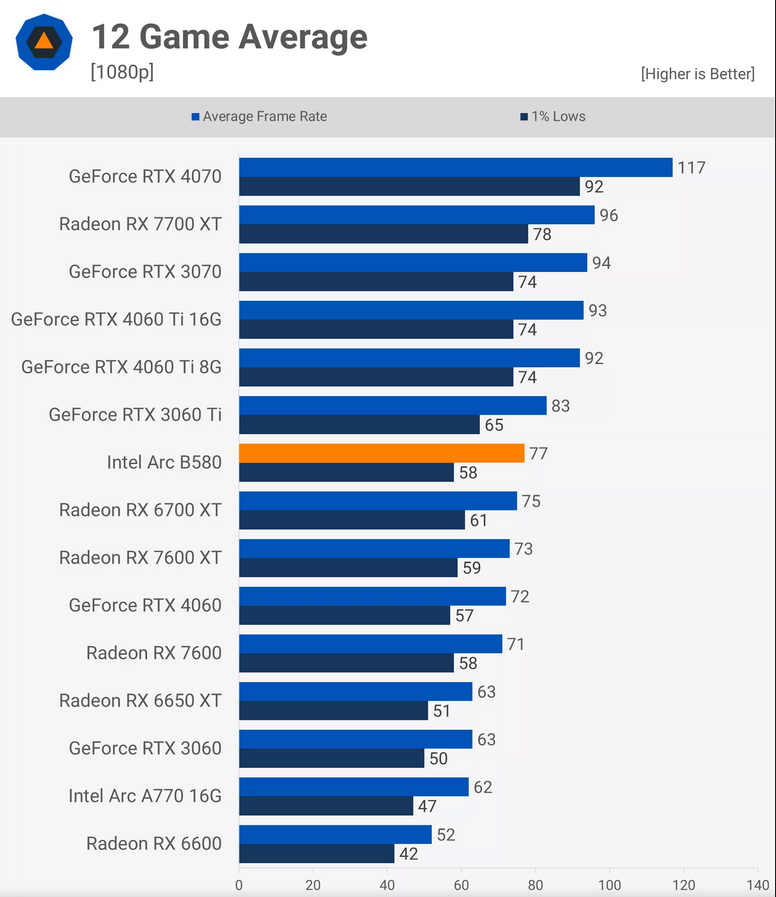
\includegraphics[width=0.9\linewidth]{4xDM/gpu.png}
\end{figure}
\end{multicols}


\subsection*{Recherche documentaire}

L'objectif de la deuxième partie est de regarder sur Internet les contraintes et les prix pour monter ce PC.

Pour se faire, nous allons devoir faire attention à ne pas dépasser le budget et prendre du matériel qui n'est pas en rupture de stock. 

\begin{enumerate}
  \item[1.] Vous pouvez directement chercher sur le site LDLC dans les différentes parties. Dans ce cas, un tri par \textbf{Top des ventes} peut être intéressant. 
  
  \url{https://www.ldlc.com/informatique/pieces-informatique/cint4197/} \\
  
   \item[2.] Vous pouvez utiliser l'outil \textbf{Le configurateur}.   Avantage du configurateur, ce dernier vous propose directement des composants compatibles une fois le choix du processeur réalisé. 
  
  \url{https://www.ldlc.com/configurateur-pc/}

\end{enumerate}

\subsection*{1. Carte Graphique :} 

Malheureusement, la carte graphique Intel Arc B580 n'est pas disponible à l'achat. Nour préfère se tourner vers une : GeForce RTX 4060 à 379 \euro{}.

\begin{itemize}[label={$\bullet$}]
  \item ASUS Dual GeForce RTX 4060 EVO OC Edition 8GB - 379 \euro{}. \newline \url{https://www.ldlc.com/fiche/PB00615606.html} \\
\end{itemize}

\newpage

\textbf{Pour le reste des achats, je vous laisse le choix dans la limite du budget total de 1200 \euro{} mais je vous impose certaines contraintes de performances.} \\


\subsection*{2. Boîtier et Alimentation :} 

\begin{itemize}[label={$\bullet$}]
  \item Un boîtier : choix libre :  \dotfill
  \item Une alimentation : au moins 550W :  \dotfill
\end{itemize} 

\subsection*{3. SSD } 

Pour le stockage des données sur votre ordinateur, vous devez prendre au moins un disque SSD : \textbf{PCIe NVMe 1 To}. Pour ceux qui le souhaite, il est possible d'ajouter un HDD de 1 To mais cela n'est pas obligatoire. 

\begin{itemize}[label={$\bullet$}]
  \item SSD : choix libre :  \dotfill
  \item HDD (faculatatif) :  \dotfill
\end{itemize} 

\subsection*{4. La carte mère et le processeur} 

La carte mère relie tous les composants de votre ordinateur. Elle joue un rôle centrale pour son fonctionnement. On lui attache obligatoirement un processeur afin de pouvoir réaliser des calculs.\\

Pour simplifier la situation, il existe deux grandes marques de processeurs qui sont en concurrence : Intel et AMD. \\

Vous avez le choix de la marque mais vous devez respecter les contraintes : \textbf{Le processeur et la carte mère doivent être compatible ; Au moins 6 cores ; Une fréquence CPU d'au moins 3,4 GHz.}

\begin{itemize}[label={$\bullet$}]
  \item Carte Mère :  \dotfill
  \item Processeur :  \dotfill
\end{itemize} 


\subsection*{5. Mémoire Vive} 

Les barettes de mémoire vive sont le plus souvent vendues par deux. Il est demandé de prendre \textbf{au moins 32 Go ($2 \times 16$ Go) de DDR5}. Attention, celles-ci doivent compatible avec la carte mère. 

\begin{itemize}[label={$\bullet$}]
  \item RAM :  \dotfill
\end{itemize} 


\subsection*{Prix du PC gamer} 

Calculer la somme d'argent nécessaire pour l'achat de ce PC avec vos composants.

\Pointilles[2]

\horrule{2px}

\begin{center}
  \textbf{Le devoir maison est à rendre pour la semaine de la rentrée.}
\end{center}

\begin{itemize}
  \item Il est possible de le rendre au format numérique sur l'ENT. 
  \begin{itemize}[label={$\bullet$}]
    \item au format texte avec LibreOffice Writer ou Microsoft Word.  
    \item au format image en réalisant une impression écran des composants / récapitulatif si vous avez utilisé l'outil "Le configurateur".
  \end{itemize}
  \item Il est possible de le rendre au format papier et dans ce cas il est demandé d'écrire : \\
  \textbf{les références exactes du produit et le prix} comme dans l'exemple de la carte graphique. 
\end{itemize} 

\end{document}